\documentclass[a4paper]{article}
\usepackage[T1]{fontenc}
\usepackage[english]{babel}
\usepackage{clrscode4e} % Algorithm template from Introduction to Algorithms 4th
\usepackage[left=2cm,right=2cm,top=1cm,bottom=2cm]{geometry} % page settings
\usepackage{amsthm, amsmath, amssymb} % provides many mathematical environments & tools
\usepackage{tikz} % draw pictures
\usepackage{tabularray}
\usepackage[noend]{algorithmic}
\usepackage{tabularx}
\usepackage{algorithm}
\usepackage{arydshln}
\usepackage{forest}
% rotation
\usepackage{adjustbox}
\usepackage{array}
\usepackage{ifthen}
% figure caption
\usepackage{caption}
\usepackage{subfig}
\usepackage{graphicx,wrapfig,lipsum}
% arrays and matrices
\usepackage{nicematrix}
% line change inside cells
\usepackage{makecell}
\usepackage{datetime}
%-----------------------------------------------------------
% Custom commands
%-----------------------------------------------------------
\newenvironment{hashtable}[1][]
  {\begin{tabular}[#1]{
     @{}
     > {\small} r <{\normalsize~\rlap{\fbox{\strut~~}}$~~\rightarrow$~}
     @{} l @{}}}
  {\end{tabular}}

\tikzset{
node of list/.style = {
             draw,
             fill=orange!20,
             minimum height=6mm,
             minimum width=6mm,
             node distance=6mm
   },
link/.style = {
     -stealth,
     shorten >=1pt
     },
array element/.style = {
    draw, fill=white,
    minimum width = 6mm,
    minimum height = 10mm
  }
}

\def\LinkedList#1{%
  \foreach \element in \list {
     \node[node of list, right = of aux, name=ele] {\element};
     \draw[link] (aux) -- (ele);
     \coordinate (aux) at (ele.east);
  }
}

\usetikzlibrary{positioning,matrix, arrows.meta}
\tikzset{box/.style={draw, thick, minimum width=1cm, minimum height=1cm}}

\newcommand{\Mod}[1]{\ (\mathrm{mod}\ #1)}

\newenvironment{solution}
  {\begin{proof}[Solution]}
  {\end{proof}}
\renewcommand{\qedsymbol}{\rule{0.7em}{0.7em}}

\makeatletter
\renewenvironment{proof}[1][\proofname]{%
  \par\pushQED{\qed}\normalfont%
  \topsep6\p@\@plus6\p@\relax
  \trivlist\item[\hskip\labelsep\bfseries#1\@addpunct{.}]%
  \ignorespaces
}{%
  \popQED\endtrivlist\@endpefalse
}
\makeatother
\setlength{\parindent}{0mm}

%-----------------------------------------------------------
% Document
%-----------------------------------------------------------
\begin{document}

\title{Algorithms: Homework 3}
\author{Li-Yuan Wei}
% day-month-year
\newdate{date}{14}{6}{2023}
\date{\displaydate{date}}
\maketitle

\subsection*{Problem 1}
Give an $\mathcal{O}(n^2)$-time algorithm to find the longest monotonically increasing subsequence of $n$ numbers.
\begin{solution}
  Psuedocode for an $\mathcal{O}(n^2)$-time algorithm:\\
\noindent
\begin{tabularx}{\textwidth}{>{\footnotesize}rX@{}}
  \\[-1.5ex] \hline
  \multicolumn{2}{@{}l}{\refstepcounter{algorithm}\label{mono-n-square} $\proc{LONGEST-INCREASING-SUBSEQUENCE}(A, n)$} \\
  \hline
  1: & $B = \proc{MERGE-SORT(A)}$ \Comment $B$ is a sorted copy of $A$ in ascending order\\
  2: & $C[n+1, n+1]$ \Comment create 2-D array $C$ with $val, dir$ fields\\
  3: & \For $i \gets 0$ \To $n$ \\
  4: & \quad $C[i][0] = 0$ \\
  5: & \For $j \gets 0$ \To $n$ \\
  6: & \quad $C[0][j] = 0$ \\
  7: & \For $i \gets 1$ \To $n$ \\
  8: & \quad \For $j \gets 1$ \To $n$ \\
  9: & \quad \quad \Do \If $B[i] \le A[j]$ \\
  10: & \quad \quad \quad $C[i][j].val = C[i - 1][j - 1].val + 1$ \\
  11: & \quad \quad \quad $C[i][j].dir = \nwarrow$ \\
  12: & \quad \quad \textbf{else} \Comment $B[i] > A[j]$ no increasing\\
  13: & \quad \quad \quad \If $C[i - 1][j].val < C[i][j - 1].val$ \\
  14: & \quad \quad \quad \quad $C[i][j].val = C[i][j - 1].val$ \\
  15: & \quad \quad \quad \quad $C[i][j].dir = \leftarrow$ \\
  16: & \quad \quad \quad \textbf{else} \\
  17: & \quad \quad \quad \quad $C[i][j].val = C[i - 1][j].val$ \\
  18: & \quad \quad \quad \quad $C[i][j].dir = \uparrow$ \\
  19: & \Return $C$ \Comment $C[n][n].val$ is the length of the longest increasing subsequence of $n$\\
\hline
\\ [-0.2cm]
\end{tabularx}
Line 1 has time complexity of merge sort, which is $\mathcal{O}(n \lg n)$. Line 2 has constant time complexity. Line 3-7 has time complexity of $\mathcal{O}(n)$. Line 6-18 has time complexity of $\mathcal{O}(n^2)$. Thus, the overall time comlexity is $\mathcal{O}(n^2)$.
\end{solution}

\subsection*{Problem 2}
Find an optimal solution to the following activity selection problem:

\begin{figure}[H]
\centering
\begin{minipage}{5cm}
\centering
$\begin{NiceArray}{*{10}{c}}[first-row, first-col, hvlines]
\CodeBefore
\Body
i  & 1 & 2 & 3 & 4 & 5 & 6 & 7 & 8 & 9 & 10\\
s_i & 1 & 3 & 2 & 3 & 5 & 8 & 7 & 10 & 5 & 11\\
f_i & 3 & 4 & 5 & 6 & 8 & 9 & 11 & 12 & 14 & 15
\end{NiceArray}$
\end{minipage}
\end{figure}

\begin{solution}
The optimal solution is to chose the following events: <1, 2, 5, 6, 8>.
\end{solution}


\subsection*{Problem 3}
Not just any greedy approach to the activity-selection problem produces a maximum-size set of mutually compatible activities. (a) Give an example to show that the approach of selecting the activity of least duration from those that are compatible with previously selected activities does not work. (b) Do the same for the approaches of always selecting the compatible activity that overlaps with the fewest other remaining activities by selecting the compatible remaining activity with the earliest start time.

\begin{figure}[H]
\begin{minipage}{8cm}
\centering
$\begin{NiceArray}{*{5}{c}}[first-row, first-col, hvlines]
\CodeBefore
\Body
i  & 1 & 2 & 3 & 4 & 5 \\
s_i & 1 & 3 & 5 & 7 & 9 \\
f_i & 5 & 6 & 9 & 10 & 13 \\
\end{NiceArray}$
\caption{(a) select least duration}
\end{minipage}
\qquad
\begin{minipage}{8cm}
\centering
$\begin{NiceArray}{*{5}{c}}[first-row, first-col, hvlines]
\CodeBefore
\Body
i  & 1 & 2 & 3 & 4 & 5 \\
s_i & 1 & 2 & 3 & 6 & 8 \\
f_i & 3 & 4 & 5 & 7 & 9 \\
\end{NiceArray}$
\caption{(b) select fewest overlaps}
\end{minipage}
\end{figure}

\begin{solution}
(a) By selecting event that has the least duration, we will pick events 2(3 - 6) and 4(7 - 10). However, if we choose events based on their earliest finish time, we will pick events 1(1 - 5), 3(5 - 9) and 5(9 - 13). \\
(b) By selecting event that has the fewest overlaps, we will pick events 4(6 - 7) and 5(8 - 9), since these two events do not overlap with other events. Yet, the optimal solution should choose events 1(1 - 3), 3(3 - 5), 4(6 - 7) and 5(8 - 9).
\end{solution}

\subsection*{Problem 4}
Give a dynamic-programming solution to the 0-1 knapsack problem that runs in $\mathcal{O}(nW)$ time, where $n$ is number of items and $W$ is the maximum weight of items that the thief can put in his knapsack. Note that $W$, as well as all the weights of the involved items are integers.
\begin{solution}
  Psuedocode for an $\mathcal{O}(nW)$-time algorithm, where $A$ is the array of $n$ items with $val, weight$ fields:\\
\noindent
\begin{tabularx}{\textwidth}{>{\footnotesize}rX@{}}
  \\[-1.5ex] \hline
  \multicolumn{2}{@{}l}{\refstepcounter{algorithm}\label{0-1-knapsack} $\proc{KNAPSACK-DP}(A, W, n)$} \\
  \hline
  1: & $C[n+1, W+1]$ \Comment create 2-D array $C$ with $val$ field\\
  2: & \For $i \gets 0$ \To $n$ \\
  3: & \quad $C[i][0].val = 0$ \Comment initialization $j$ from $0$ to $n$\\
  4: & \For $j \gets 0$ \To $W$ \\
  5: & \quad $C[0][j].val = 0$ \Comment initialization $i$ from $0$ to $W$\\
  6: & \For $i \gets 1$ \To $n$ \\
  7: & \quad \For $j \gets 1$ \To $W$ \\
  8: & \quad \quad \If $A[i].weight > j$ \Comment current item's weight is greater than the knapsack capacity\\
  9: & \quad \quad \quad $C[i][j].val = C[i - 1][j].val$ \Comment get the value of previous $i - 1$ items\\
 10: & \quad \quad \textbf{else} \\
 11: & \quad \quad \quad \Comment $C[i - 1][j].val$: value of no additional item \\
 12: & \quad \quad \quad \Comment $C[i - 1][j - A[i].weight] + A[i].val$: value of add $A[i]$ into knapsack\\
 13: & \quad \quad \quad $C[i][j].val = MAX(C[i - 1][j].val, C[i - 1][j - A[i].weight] + A[i].val)$\\
 14: & \Return $C$ \Comment $C[n][W].val$ has the maximum value of knapsack\\
\hline
\\ [-0.2cm]
\end{tabularx}
Line 1 has constant time complexity. Line 3-4 has time complexity of $\mathcal{O}(n)$, while line 5-6 has time complexity of $\mathcal{O}(W)$. Line 6-13 has time complexity of $\mathcal{O}(nW)$. Thus, the overall time comlexity is $\mathcal{O}(nW)$.
\end{solution}

\subsection*{Problem 5}
Assume there are only 7 characters A, B, C, D, E, F and G in a document, with occurrences of 6, 4, 8, 3, 2, 1 and 5, respectively. Please calculate the total number of bits of this document after applying the Huffman coding.

\begin{minipage}{5cm}
\begin{align*}
  \text{C: 8 }& |\ 11 \\
  \text{A: 6 }& |\ 01 \\
  \text{G: 5 }& |\ 101 \\
  \text{B: 4 }& |\ 100 \\
  \text{D: 3 }& |\ 001 \\
  \text{E: 2 }& |\ 0000 \\
  \text{F: 1 }& |\ 0001 \\
\end{align*}
\end{minipage}
\qquad
\begin{minipage}{5cm}
\begin{figure}[H]
\centering
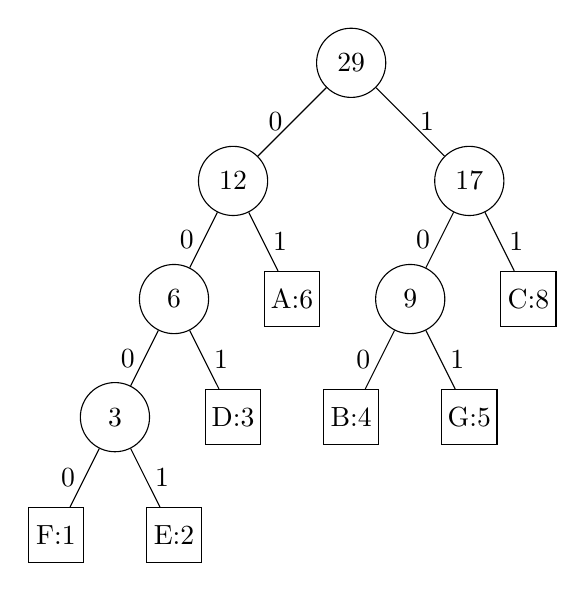
\begin{tikzpicture}[iv/.style={draw,circle,minimum size=25pt,inner
sep=0pt,text=black},ev/.style={draw,rectangle,minimum
size=20pt,inner sep=0pt,text=black}]
\node[iv]{29}
  child {node[iv]{12}
          child {node[iv]{6}
                 child {node[iv]{3}
                        child {node[ev]{F:1}
                          edge from parent node[left]{0}
                        }
                        child {node[ev]{E:2}
                          edge from parent node[right]{1}
                        }
                  edge from parent node[left]{0}
                 }
                 child {node[ev]{D:3}
                  edge from parent node[right]{1}
                 }
            edge from parent node[left]{0}
          }
          child {node[ev]{A:6}
            edge from parent node[right]{1}
          }
          edge from parent node[left]{0}
          }
  child [missing]
  child {node[iv]{17}
            child {node[iv]{9}
              child {node[ev]{B:4}
                edge from parent node[left]{0}
              }
              child {node[ev]{G:5}
                edge from parent node[right]{1}
              }
              edge from parent node[left]{0}
            }
          child {node[ev]{C:8}
            edge from parent node[right]{1}
          }
          edge from parent node[right]{1}
        };
\end{tikzpicture}
\caption{Huffman code tree}
\end{figure}
\end{minipage}

\begin{solution}
  total bits: $1 \cdot 4 + 2 \cdot 4 + 3 \cdot 3 + 4 \cdot 3 + 5 \cdot 3 + 6 \cdot 2 + 8 \cdot 2 = 76$
\end{solution}

\subsection*{Problem 6}
Represent the graph on the right by adjacency-matrix and adjacency-list.
\begin{solution}
\begin{figure}[H]
\centering
\begin{minipage}{5cm}
\centering
$\begin{NiceArray}{*{5}{c}}[first-row, first-col, hvlines, name=amatrix]
  & 1 & 2 & 3 & 4 & 5 \\
1 & 0 & 1 & 0 & 1 & 0 \\
2 & 1 & 0 & 1 & 1 & 0 \\
3 & 0 & 1 & 0 & 0 & 1 \\
4 & 1 & 1 & 0 & 0 & 1 \\
5 & 0 & 0 & 1 & 1 & 0 \\
\end{NiceArray}$
\caption{adjacency-matrix}
\end{minipage}
\qquad
\begin{minipage}{5cm}
\centering
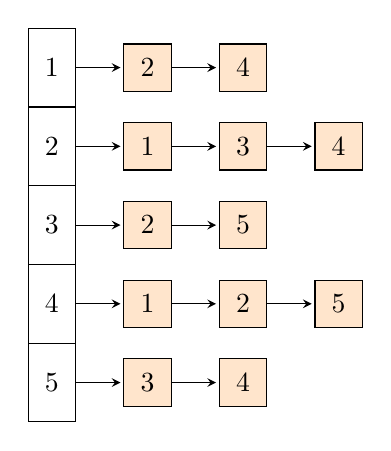
\begin{tikzpicture}
  \foreach \index/\list in {1/{2, 4}, 2/{1, 3, 4}, 3/{2, 5}, 4/{1, 2, 5}, 5/{3, 4}} {
   \node[array element] (aux) at (0,-\index) {\index};
   \LinkedList{\list}
}
\end{tikzpicture}
\caption{adjacency-list}
\end{minipage}
\end{figure}
\end{solution}

\subsection*{Problem 7}
Show the $d$ and $\pi$ values that result from running the breadth-first search on the same graph using vertex 3 as the source.
\begin{figure}[H]
\centering
\begin{minipage}{5cm}
\centering
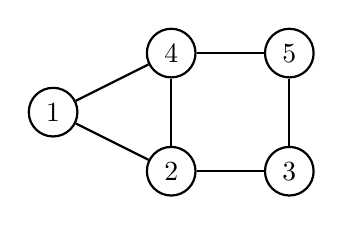
\begin{tikzpicture}[anchor=base, node distance={15mm}, thick, main/.style = {draw, circle}]
\node[main] (3) {$3$};
\node[main] (5) [above of=3]{$5$};
\node[main] (4) [left of=5]{$4$};
\node[main] (2) [left of=3]{$2$};
%\node[main] (1) [above left of=2]{$1$};
\path (2) -- (4) node[midway, left of=2, circle, thick, draw] (1) {$1$};

\draw[] (1) -- (4);
\draw[] (1) -- (2);
\draw[] (2) -- (4);
\draw[] (2) -- (3);
\draw[] (3) -- (5);
\draw[] (4) -- (5);
\end{tikzpicture}
\caption{Original Graph}
\end{minipage}
\qquad
\begin{minipage}{5cm}
\centering
$\begin{NiceArray}{*{5}{c}}[first-row, first-col, hvlines]
\CodeBefore
\Body
 v & 1 & 2 & 3 & 4 & 5 \\
 d & 2 & 1 & 0 & 2 & 1 \\
 \pi & 2 & 3 & \textbf{NIL} & 2 & 3
\end{NiceArray}$
\end{minipage}
\end{figure}

\begin{solution}
$v$ stands for verticies in the graph. $d$ is the search distance, while $\pi$ is vertex $v$'s parent node. Vertex 3 is the starting point, thus, it has no parent node.
\end{solution}

\subsection*{Problem 8}
(a) Show how depth-first search works on the graph at the bottom. Assume that the for loop of lines 5—7 of the DFS procedure considers the vertices in alphabetical order, and assume that each adjacency list is ordered alphabetically. Show the discovery and finishing time for each vertex, and show the classification of each edge. (b) According to (a), show the corresponding topological sort of this graph.
\begin{figure}[H]
\centering
\begin{minipage}{5cm}
\centering
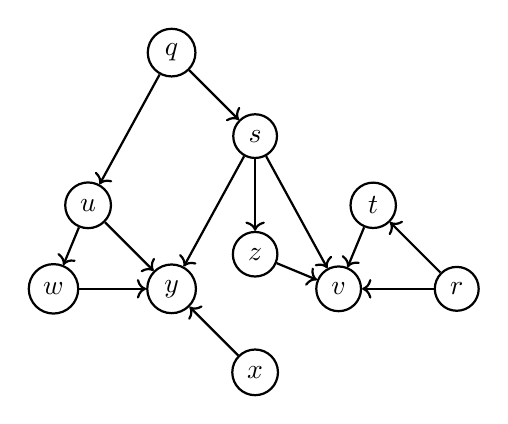
\begin{tikzpicture}[node distance={15mm}, thick, main/.style = {draw, circle}, name=p8]
\node[main] (x) {$x$};
\node[main] (y) [above left of=x]{$y$};
\node[main] (w) [left of=y]{$w$};
\node[main] (v) [above right of=x]{$v$};
\node[main] (r) [right of=v]{$r$};
\node[main] (z) [above of=x]{$z$};
\node[main] (s) [above of=z]{$s$};
\node[main] (t) [above left of=r]{$t$};
\node[main] (u) [above left of=y]{$u$};
\node[main] (q) [above left of=s]{$q$};

\draw[->] (x) -- (y);
\draw[->] (w) -- (y);
\draw[->] (u) -- (y);
\draw[->] (s) -- (y);
\draw[->] (u) -- (w);
\draw[->] (s) -- (z);
\draw[->] (s) -- (v);
\draw[->] (z) -- (v);
\draw[->] (t) -- (v);
\draw[->] (r) -- (v);
\draw[->] (r) -- (t);
\draw[->] (q) -- (u);
\draw[->] (q) -- (s);
\end{tikzpicture}
\caption{Original Graph}
\end{minipage}
\qquad
\begin{minipage}{8cm}
\centering
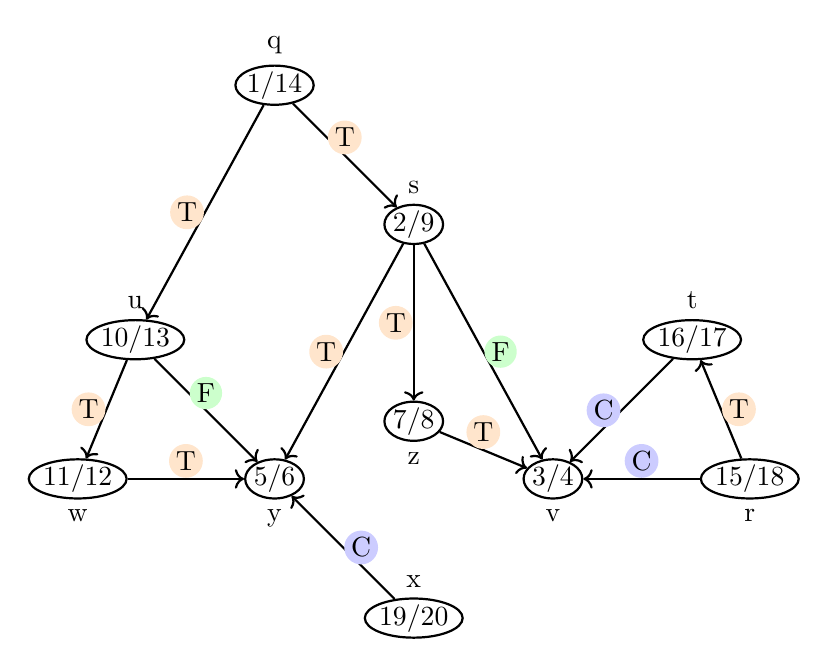
\begin{tikzpicture}[node distance={25mm}, thick, main/.style = {draw, ellipse, inner sep=0pt}, name=p8]
\node[main] (x8) [label=x]{19/20};
\node[main] (y8) [above left of=x8, label=below:y]{5/6};
\node[main] (w8) [left of=y8, label=below:w]{11/12};
\node[main] (v8) [above right of=x8, label=below:v]{3/4};
\node[main] (r8) [right of=v8, label=below:r]{15/18};
\node[main] (z8) [above of=x8, label=below:z]{7/8};
\node[main] (s8) [above of=z8, label=s]{2/9};
\node[main] (t8) [above right of=v8, label=t]{16/17};
\node[main] (u8) [above left of=y8, label=u]{10/13};
\node[main] (q8) [above left of=s8, label=q]{1/14};

\draw[->] (x8) -- node[circle,inner sep=0.8, fill=blue!20, right]{C}(y8);
\draw[->] (w8) -- node[circle,inner sep=0.8, fill=orange!20, above]{T}(y8);
\draw[->] (u8) -- node[circle,inner sep=0.8, fill=green!20, above]{F}(y8);
\draw[->] (s8) -- node[circle,inner sep=0.8, fill=orange!20, left]{T}(y8);
\draw[->] (u8) -- node[circle,inner sep=0.8, fill=orange!20, left]{T}(w8);
\draw[->] (s8) -- node[circle,inner sep=0.8, fill=orange!20, left]{T}(z8);
\draw[->] (s8) -- node[circle,inner sep=0.8, fill=green!20, right]{F}(v8);
\draw[->] (z8) -- node[circle,inner sep=0.8, fill=orange!20, above]{T}(v8);
\draw[->] (t8) -- node[circle,inner sep=0.8, fill=blue!20, left]{C}(v8);
\draw[->] (r8) -- node[circle,inner sep=0.8, fill=blue!20, above]{C}(v8);
\draw[->] (r8) -- node[circle,inner sep=0.8, fill=orange!20, right]{T}(t8);
\draw[->] (q8) -- node[circle,inner sep=0.8, fill=orange!20, left]{T}(u8);
\draw[->] (q8) -- node[circle,inner sep=0.8, fill=orange!20, above]{T} (s8);
\end{tikzpicture}
\caption{(a) DFS with discovery, finish time and edge classification}
\end{minipage}
\end{figure}

\begin{figure}[H]
\centering
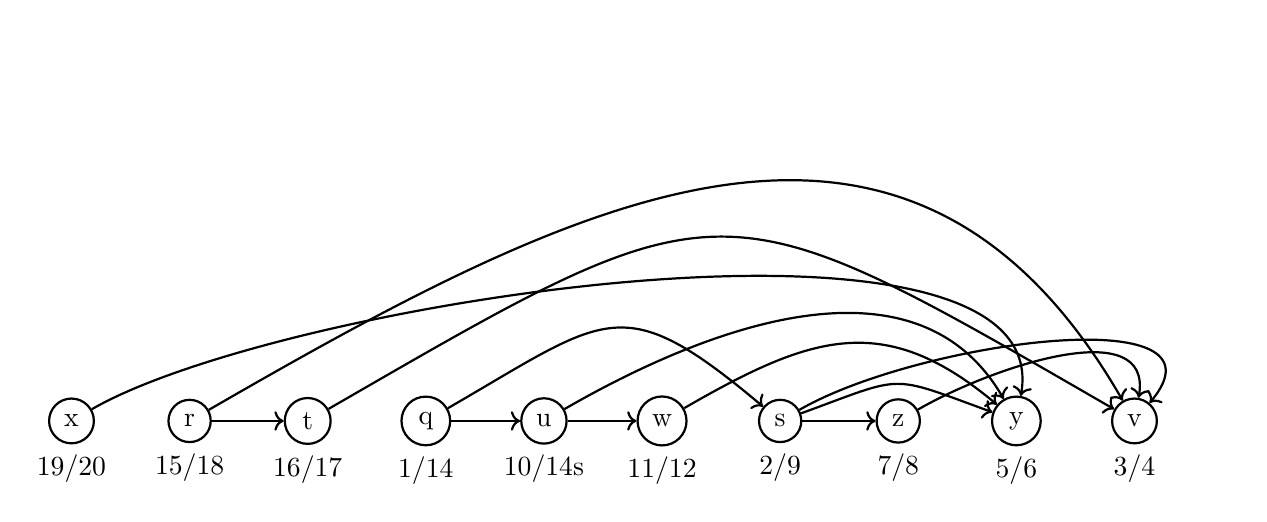
\begin{tikzpicture}[node distance={15mm}, thick, main/.style = {draw, circle}, name=p82]
  \node[main] (xt) [label=below:19/20] {x};
  \node[main] (rt) [right of=xt, label=below:15/18] {r};
  \node[main] (tt) [right of=rt, label=below:16/17] {t};
  \node[main] (qt) [right of=tt, label=below:1/14] {q};
  \node[main] (ut) [right of=qt,label=below:10/14s] {u};
  \node[main] (wt) [right of=ut,label=below:11/12] {w};
  \node[main] (st) [right of=wt,label=below:2/9] {s};
  \node[main] (zt) [right of=st,label=below:7/8] {z};
  \node[main] (yt) [right of=zt,label=below:5/6] {y};
  \node[main] (vt) [right of=yt,label=below:3/4] {v};

  \draw[->] (qt) -- (ut);
  \draw[->] (ut) -- (wt);
  \draw[->] (st) -- (zt);
  \draw[->] (rt) -- (tt);
  \draw[->] (qt) to [out=30, in=140, looseness=1.5] (st);
  \draw[->] (wt) to [out=30, in=140, looseness=1.2] (yt);
  \draw[->] (ut) to [out=30, in=120, looseness=1] (yt);
  \draw[->] (st) to [out=20, in=160, looseness=1.5] (yt);
  \draw[->] (xt) to [out=30, in=80, looseness=0.6] (yt);
  \draw[->] (zt) to [out=30, in=80, looseness=1] (vt);
  \draw[->] (st) to [out=30, in=50, looseness=1] (vt);
  \draw[->] (rt) to [out=30, in=120, looseness=1.2] (vt);
  \draw[->] (tt) to [out=30, in=150, looseness=1.5] (vt);

\end{tikzpicture}
\caption{(b) topological sort with decreasing finish time order}
\end{figure}

\subsection*{Problem 9}
Find the strongest components of the following graph:
\begin{figure}[H]
\centering
\begin{minipage}{8cm}
\centering
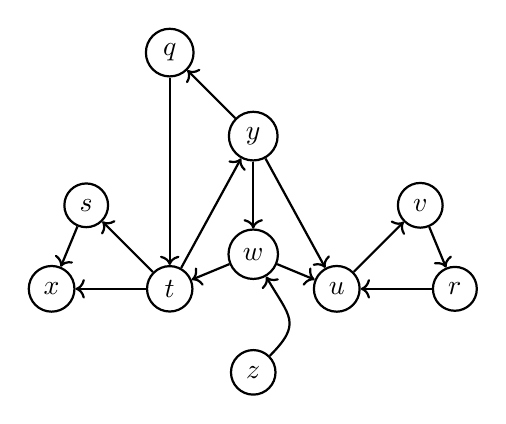
\begin{tikzpicture}[node distance={15mm}, thick, main/.style = {draw, circle}, name=p9]
\node[main] (z9) {$z$};
\node[main] (w9) [above of=z9]{$w$};2
\node[main] (t9) [above left of=z9]{$t$};
\node[main] (u9) [above right of=z9]{$u$};
\node[main] (y9) [above of=w9]{$y$};
\node[main] (q9) [above left of=y9]{$q$};
\node[main] (x9) [left of=t9]{$x$};
\node[main] (s9) [above left of=t9]{$s$};
\node[main] (v9) [above right of=u9]{$v$};
\node[main] (r9) [right of=u9]{$r$};

\draw[->] (z9) to [out=45,in=300,looseness=1.5] (w9);
\draw[->] (w9) -- (u9);
\draw[->] (w9) -- (t9);
\draw[->] (y9) -- (w9);
\draw[->] (y9) -- (q9);
\draw[->] (y9) -- (u9);
\draw[->] (t9) -- (y9);
\draw[->] (q9) -- (t9);
\draw[->] (t9) -- (s9);
\draw[->] (s9) -- (x9);
\draw[->] (t9) -- (x9);
\draw[->] (r9) -- (u9);
\draw[->] (v9) -- (r9);
\draw[->] (u9) -- (v9);

\end{tikzpicture}
\caption{Original Graph}
\label{fig:p9}
\end{minipage}
\qquad
\begin{minipage}{8cm}
\centering
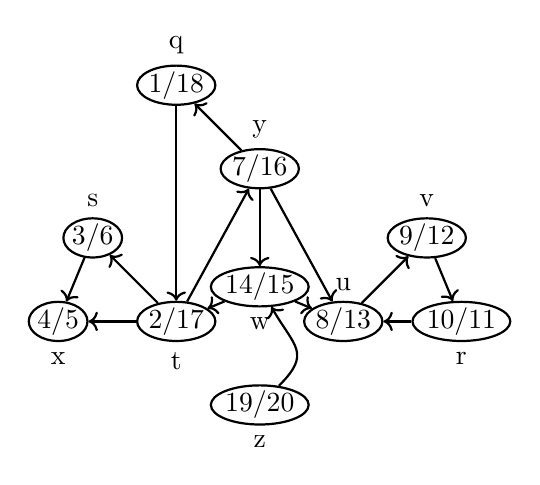
\begin{tikzpicture}[node distance={15mm}, thick, main/.style = {draw, ellipse, inner sep=0pt}, name=p9d]
\node[main] (z9) [label=below:z]{19/20};
\node[main] (w9) [above of=z9, label=below:w]{14/15};
\node[main] (t9) [above left of=z9, label=below:t]{2/17};
\node[main] (u9) [above right of=z9, label=u]{8/13};
\node[main] (y9) [above of=w9, label=y]{7/16};
\node[main] (q9) [above left of=y9, label=q]{1/18};
\node[main] (x9) [left of=t9, label=below:x]{4/5};
\node[main] (s9) [above left of=t9, label=s]{3/6};
\node[main] (v9) [above right of=u9, label=v]{9/12};
\node[main] (r9) [right of=u9, label=below:r]{10/11};

\draw[->] (z9) to [out=45,in=300,looseness=1.5] (w9);
\draw[->] (w9) -- (u9);
\draw[->] (w9) -- (t9);
\draw[->] (y9) -- (w9);
\draw[->] (y9) -- (q9);
\draw[->] (y9) -- (u9);
\draw[->] (t9) -- (y9);
\draw[->] (q9) -- (t9);
\draw[->] (t9) -- (s9);
\draw[->] (s9) -- (x9);
\draw[->] (t9) -- (x9);
\draw[->] (r9) -- (u9);
\draw[->] (v9) -- (r9);
\draw[->] (u9) -- (v9);

\end{tikzpicture}
\caption{First DFS}
\label{fig:dfs1}
\end{minipage}
\qquad
\begin{minipage}{8cm}
\centering
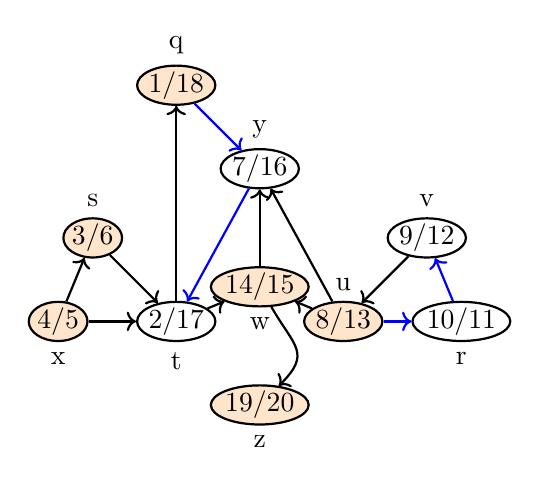
\begin{tikzpicture}[node distance={15mm}, thick, main/.style = {draw, ellipse, inner sep=0pt}, name=p9d]
\node[main] (z9) [fill=orange!20, label=below:z]{19/20};
\node[main] (w9) [fill=orange!20, above of=z9, label=below:w]{14/15};
\node[main] (t9) [above left of=z9, label=below:t]{2/17};
\node[main] (u9) [fill=orange!20, above right of=z9, label=u]{8/13};
\node[main] (y9) [above of=w9, label=y]{7/16};
\node[main] (q9) [fill=orange!20, above left of=y9, label=q]{1/18};
\node[main] (x9) [fill=orange!20,left of=t9, label=below:x]{4/5};
\node[main] (s9) [fill=orange!20,above left of=t9, label=s]{3/6};
\node[main] (v9) [above right of=u9, label=v]{9/12};
\node[main] (r9) [right of=u9, label=below:r]{10/11};

\draw[<-] (z9) to [out=45,in=300,looseness=1.5] (w9);
\draw[<-] (w9) -- (u9);
\draw[<-] (w9) -- (t9);
\draw[<-] (y9) -- (w9);
\draw[<-, blue] (y9) -- (q9);
\draw[<-] (y9) -- (u9);
\draw[<-, blue] (t9) -- (y9);
\draw[<-] (q9) -- (t9);
\draw[<-] (t9) -- (s9);
\draw[<-] (s9) -- (x9);
\draw[<-] (t9) -- (x9);
\draw[<-, blue] (r9) -- (u9);
\draw[<-, blue] (v9) -- (r9);
\draw[<-] (u9) -- (v9);

\end{tikzpicture}
\caption{Second DFS with Transpose Graph}
\label{fig:dfs2}
\end{minipage}
\qquad
\begin{minipage}{8cm}
\centering
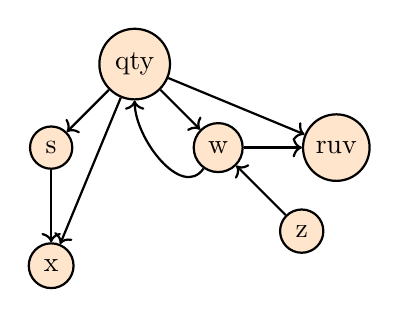
\begin{tikzpicture}[node distance={15mm}, thick, main/.style = {draw, circle}, name=p9scc]
\node[main] (z9) [fill=orange!20]{z};
\node[main] (w9) [fill=orange!20, above left of=z9]{w};
\node[main] (u9) [fill=orange!20, right of=w9]{ruv};
\node[main] (q9) [fill=orange!20, above left of=w9]{qty};
\node[main] (s9) [fill=orange!20, below left of=q9]{s};
\node[main] (x9) [fill=orange!20, below of=s9]{x};

\draw[->] (s9) -- (x9);
\draw[->] (q9) -- (s9);
\draw[->] (q9) -- (x9);
\draw[->] (q9) -- (w9);
\draw[->] (z9) -- (w9);
\draw[->] (q9) -- (u9);
\draw[->] (w9) -- (u9);
\draw[->] (w9) to [out=235, in=270] (q9);
\end{tikzpicture}
\caption{Strongly Connected Components}
\label{fig:scc}
\end{minipage}
\end{figure}

\begin{solution}
  Based on the graph in Figure \ref{fig:p9}, we first call DFS and get the discovery, finish time in Figure \ref{fig:dfs1}. After the first DFS call, we transpose our graph to reverse all edges and run DFS again(run with each vertex's finish time in decreasing order. In this example, DFS will run based on this order: $z$, $q$, $w$, $u$, $s$, $x$), yielding Figure \ref{fig:dfs2}. As a result, we have our strongly connected components in Figure \ref{fig:scc}.
\end{solution}

\newpage
\subsection*{Problem 10}
Find the minimal spanning tree of the following graph, using (a) Kruskal’s algorithm, (b) Prim’s algorithm (using q as the starting vertex). Please give the selected edge in order during the spanning tree construction process
\begin{figure}[H]
\centering
\begin{minipage}{5cm}
\centering
\begin{tikzpicture}[node distance={15mm}, thick, main/.style = {draw, circle}, name=p10]
\node[main] (y) [left of=w]{$y$};
\node[main] (z) {$z$};
\node[main] (w) [right of=y]{$w$};
\node[main] (x) [above of=z]{$x$};
\node[main] (s) [above right of=y]{$s$};
\node[main] (t) [above of=x]{$t$};
\node[main] (q) [above left of=t]{$q$};

\draw[] (q) -- node[midway, above left]{2}(s);
\draw[] (q) -- node[midway, above right]{9}(t);
\draw[] (s) -- node[midway, above]{6}(t);
\draw[] (s) -- node[midway, above left]{8}(y);
\draw[] (s) -- node[midway, above right]{4}(w);
\draw[] (y) -- node[midway, above]{10}(w);
\draw[] (t) -- node[midway, right]{5}(x);
\draw[] (x) -- node[midway, above]{1}(w);
\draw[] (x) -- node[midway, right]{7}(z);
\draw[] (w) -- node[midway, below left]{3}(z);
\end{tikzpicture}
\caption{Original Graph}
\label{fig:p10}
\end{minipage}
\qquad
\begin{minipage}{10cm}
\centering
\begin{tikzpicture}[node distance={15mm}, thick, main/.style = {draw, circle}]
\node[main] (y) [left of=w]{$y$};
\node[main] (z) {$z$};
\node[main] (w) [right of=y]{$w$};
\node[main] (x) [above of=z]{$x$};
\node[main] (s) [above right of=y]{$s$};
\node[main] (t) [above of=x]{$t$};
\node[main] (q) [above left of=t]{$q$};

\draw[ultra thick] (x) -- node[black, fill=orange!20, inner sep=1.5, circle, midway, above]{1}(w);
\draw[ultra thick] (q) -- node[black, fill=orange!20,  inner sep=1.5,circle, midway, above left]{2}(s);
\draw[ultra thick] (w) -- node[black, fill=orange!20, inner sep=1.5,circle, midway, below left]{3}(z);
\draw[ultra thick] (s) -- node[black, fill=orange!20,inner sep=1.5, circle, midway, above right]{4}(w);
\draw[ultra thick] (t) -- node[black, fill=orange!20,inner sep=1.5, circle, midway, right]{5}(x);
\draw[ultra thick] (s) -- node[black, fill=orange!20,inner sep=1.5, circle, midway, above left]{6}(y);

\draw[] (q) -- (t);
\draw[] (s) -- (t);
\draw[] (y) -- (w);
\draw[] (x) -- (z);
\end{tikzpicture}
\caption{Minimal Spanning Tree: Kruskal's algorithm}
\label{fig:kruskal}
\end{minipage}
\end{figure}

\begin{solution}
  Kruskal's algorithm: first sort all edges in the graph in increasing order, then pick the lowest cost edge every step until every vertex is connected to our tree. The final result is shown in Figure \ref{fig:kruskal}.
\end{solution}
\end{document}


